Hicimos la elecci�n de direcciones de iluminaci�n con el procedimiento explicado en la parte de desarrollo y obtuvimos la siguiente matriz, que tiene el numero de condicion 15.0503:
\break
\\
$\begin{pmatrix} 0.15625000  & -0.59765625 & 0.78637964\\ -0.11718750 & -0.57421875 & 0.81027151 \\ 0.03515625 & -0.44140625 & 0.89661840 \end{pmatrix}$
\break
\\
y la siguiente matriz que tiene el m�ximo numero de condici�n, 407,581:
\break
\\
$\begin{pmatrix} -0.03906250 & -0.56250000 & 0.82587400\\ -0.04296875 & -0.56250000 & 0.82567998\\ -0.04687500& -0.56250000 & 0.82546743 \end{pmatrix}$
\break
\\
Luego generamos los campos de las normales y obtuvimos los siguientes resultados:


\begin{center}
   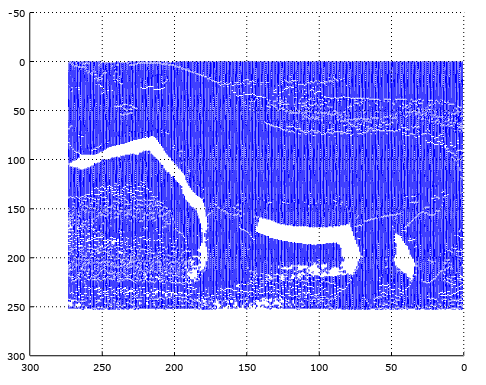
\includegraphics[scale=0.3]{caballoMax.png}
   \label{Fig. 1}
\end{center}

\begin{center}
   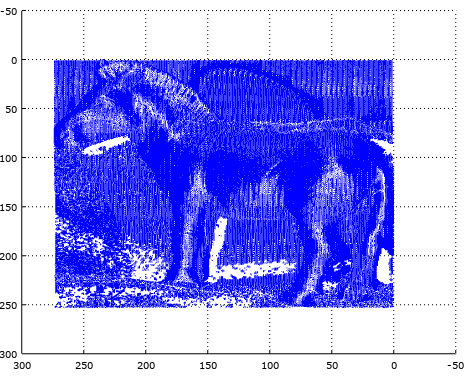
\includegraphics[scale=0.3]{caballoMin.png}
   \label{Fig. 2}
\end{center}

El siguiente grafico muestra los resultados que obtuvimos en e experimento donde comparamos las complejidades temporales del algoritmo de eliminacion de guass, la facotrizacion LU y Chelosky.

\begin{center}
   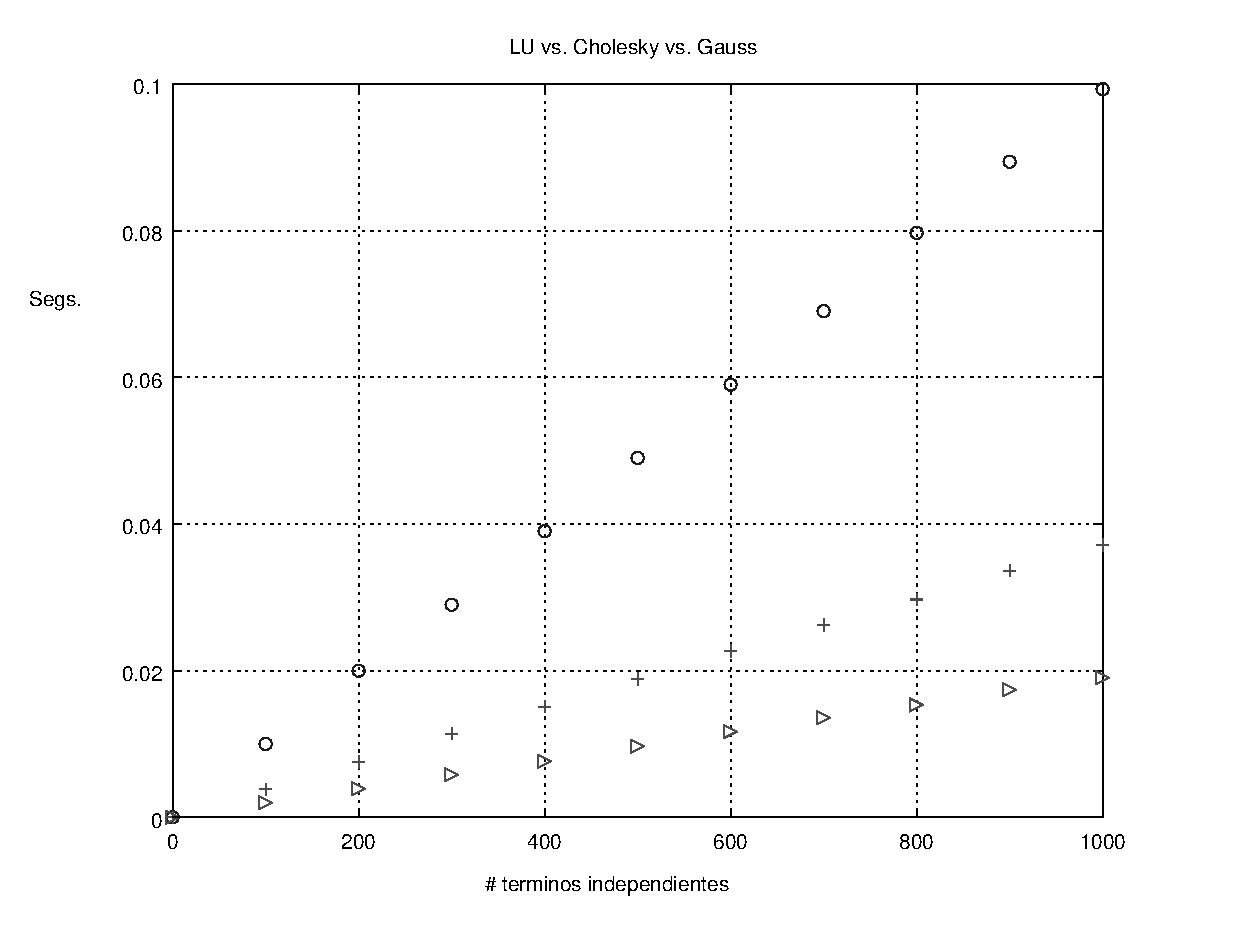
\includegraphics[scale=0.6]{LuCholeGauss.eps}
   \label{Fig. 3}
\end{center}

\indent Nuestra hip�tesis de que el numero de condici�n afecta directamente la estimaci�n de las normales se puede ver confirmada claramente en las im�gen del caballo. El campo de normales del caballo  en las figuras 1  esta estimado con la elecci�n de direcciones de iluminaci�n que causan que la matriz de la ecuaci�n 5 tanga el m�ximo numero de condici�n en comparaci�n a todas las otras posibles combinaciones de direcciones. En contraste la figura 2 utiliza la conbinaci�n de direcciones de illuminacion que generan la matriz con el mejor numero de condici�n. Esto se da porque un numero de condici�n alto implica que las direcciones de iluminaci�n est�n apuntando desde una posici�n muy similar lo cual es equivalente a tener una sola direccion para generar las normales y tambi�n las profundidades. \par
